% locking/locking.tex

\QuickQuizChapter{chp:Locking}{Locking}

The role of villain in much of the past few decades' concurrency research
literature is played by locking,
which stands accused of promoting deadlocks, convoying, starvation,
unfairness, data races, and all manner of other concurrency sins.
Interestingly enough, the role of workhorse in shared-memory parallel
software is played by, you guessed it, locking.

There are a number of reasons behind this dichotomy:

\begin{enumerate}
\item	Many of locking's sins have pragmatic design solutions that
	work well in most cases, for example:
	\begin{enumerate}
	\item	Lock hierarchies to avoid deadlock.
	\item	Deadlock-detection tools, for example, the Linux kernel's
		lockdep facility~\cite{JonathanCorbet2006lockdep}.
	\item	Locking-friendly data structures, such as
		arrays, hash tables, and radix trees, which will
		be covered in Chapter~\ref{chp:Data Structures}.
	\end{enumerate}
\item	Some of locking's sins are problems only at high levels of
	contention, levels reached only by poorly designed programs.
\item	Some of locking's sins are avoided by using other synchronization
	mechanisms in concert with locking.
	These other mechanisms include reference counters,
	statistical counters, simple non-blocking data structures, and RCU.
\item	Until quite recently, almost all large shared-memory parallel
	programs were developed in secret, so that it was difficult for
	most researchers to learn of these pragmatic solutions.
\item	All good stories need a villain, and locking has a long and
	honorable history serving as a research-paper whipping boy.
\end{enumerate}

This chapter will give an overview of a number of ways to avoid locking's
more serious sins.

\begin{figure}[tb]
\begin{center}
\resizebox{3in}{!}{\includegraphics{locking/LockingTheSlob}}
\end{center}
\caption{Locking: Villain or Slob?}
\label{fig:locking:Locking: Villain or Slob?}
\end{figure}

\begin{figure}[tb]
\begin{center}
\resizebox{3in}{!}{\includegraphics{locking/LockingTheHero}}
\end{center}
\caption{Locking: Workhorse or Hero?}
\label{fig:locking:Locking: Workhorse or Hero?}
\end{figure}

\section{Staying Alive}
\label{sec:locking:Staying Alive}

Given that locking stands accused of deadlock and starvation,
one important concern for shared-memory parallel developers is
simply staying alive.
The following sections therefore cover deadlock, livelock, starvation,
unfairness, and inefficiency.

\subsection{Deadlock}
\label{sec:locking:Deadlock}

Deadlock occurs when each of a group of threads is holding at least one
lock while at the same time waiting on a lock held by a member
of the same group.

Without some sort of external intervention, deadlock is forever.
No thread can acquire the lock it is waiting on until that
lock is released by the thread holding it, but the thread holding
it cannot release it until the holding thread acquires the lock that
it is waiting on.

\begin{figure}[tb]
\begin{center}
\resizebox{3in}{!}{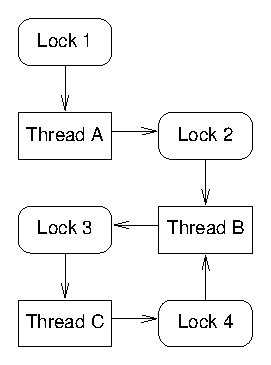
\includegraphics{locking/DeadlockCycle}}
\end{center}
\caption{Deadlock Cycle}
\label{fig:locking:Deadlock Cycle}
\end{figure}

We can create a directed-graph representation of a deadlock scenario
with nodes for threads and locks, as shown in
Figure~\ref{fig:locking:Deadlock Cycle}.
An arrow from a lock to a thread indicates that the thread holds
the lock, for example, Thread~B holds Locks~2 and 4.
An arrow from a thread to a lock indicates that the thread is waiting
on the lock, for example, Thread~B is waiting on Lock~3.

A deadlock scenario will always contain at least one deadlock cycle.
In Figure~\ref{fig:locking:Deadlock Cycle}, this cycle is
Thread~B, Lock~3, Thread~C, Lock~4, and back to Thread~B.

\QuickQuiz{}
	But the definition of deadlock only said that each thread
	was holding at least one lock and waiting on another lock
	that was held by some thread.
	How do you know that there is a cycle?
\QuickQuizAnswer{
	Suppose that there is not cycle in the graph.
	We would then have a directed acyclic graph (DAG), which would
	have at least one leaf node.

	If this leaf node was a lock, then we would have a thread
	that was waiting on a lock that wasn't held by any thread,
	which violates the definition.
	(And in this case the thread would immediately acquire the
	lock.)

	On the other hand, if this leaf node was a thread, then
	we would have a thread that was not waiting on any lock,
	again violating the definition.
	(And in this case, the thread would either be running or
	blocked on something that is not a lock.)

	Therefore, given this definition of deadlock, there must
	be a cycle in the corresponding graph.
} \QuickQuizEnd

Although there are some software environments such as database systems
that can repair an existing deadlock, this approach requires either that
one of the threads be killed or that a lock be forcibly stolen from one
of the threads.
This killing and forcible stealing can be appropriate for transactions,
but is problematic for kernel and application-level use of locking.

Kernels and applications therefore work to avoid deadlocks.
There are three major approaches,
locking hierarchies, conditional locking, and
single-lock-at-a-time designs.

Locking hierarchies order the locks and prohibit acquiring locks out
of order.
In Figure~\ref{fig:locking:Deadlock Cycle},
we might order the locks numerically, so that a thread was
forbidden from acquiring a given lock if it already held a lock
with the same or a higher number.
Thread~B has violated this hierarchy because it is attempting to
acquire Lock~3 while holding Lock~4, which permitted the deadlock
to occur.

Again, to apply a locking hierarchy, order the locks and prohibit
out-of-order lock acquisition.
In large program, it is wise to use tools to enforce your locking
hierarchy~\cite{JonathanCorbet2006lockdep}.

\begin{figure}[tbp]
{ \scriptsize
\begin{verbatim}
  1 spin_lock(&lock2);
  2 layer_2_processing(pkt);
  3 nextlayer = layer_1(pkt);
  4 spin_lock(&nextlayer->lock1);
  5 layer_1_processing(pkt);
  6 spin_unlock(&lock2);
  7 spin_unlock(&nextlayer->lock1);
\end{verbatim}
}
\caption{Protocol Layering and Deadlock}
\label{fig:locking:Protocol Layering and Deadlock}
\end{figure}

But suppose that there is no reasonable locking hierarchy.
This can happen in real life, for example, in layered network protocol stacks
where packets flow in both directions.
In the networking case, it might be necessary to hold the locks from
both layers when passing a packet from one layer to another.
Given that packets travel both up and down the protocol stack, this
is an excellent recipe for deadlock, as illustrated in
Figure~\ref{fig:locking:Protocol Layering and Deadlock}.
Here, a packet moving down the stack towards the wire must acquire
the next layer's lock out of order.
Given that packets moving up the stack away from the wire are acquiring
the locks in order, the lock acquisition in line~4 of the figure
can result in deadlock.

\begin{figure}[tbp]
{ \scriptsize
\begin{verbatim}
  1 retry:
  2   spin_lock(&lock2);
  3   layer_2_processing(pkt);
  4   nextlayer = layer_1(pkt);
  5   if (!spin_trylock(&nextlayer->lock1)) {
  6     spin_unlock(&lock2);
  7     spin_lock(&nextlayer->lock1);
  8     spin_lock((&lock2);
  9     if (layer_1(pkt) != nextlayer) {
 10       spin_unlock(&nextlayer->lock1);
 11       spin_unlock((&lock2);
 12       goto retry;
 13     }
 14   }
 15   layer_1_processing(pkt);
 16 spin_unlock(&lock2);
 17 spin_unlock(&nextlayer->lock1);
\end{verbatim}
}
\caption{Avoiding Deadlock Via Conditional Locking}
\label{fig:locking:Avoiding Deadlock Via Conditional Locking}
\end{figure}

One way to avoid deadlocks in this case is to impose a locking hierarchy,
but when it is necessary to acquire a lock out of order, acquire it
conditionally, as shown in
Figure~\ref{fig:locking:Avoiding Deadlock Via Conditional Locking}.
Instead of unconditionally acquiring the layer-1 lock, line~5
conditionally acquires the lock using the \co{spin_trylock()} primitive.
This primitive acquires the lock immediately if the lock is available
(returning non-zero), and otherwise returns zero without acquiring the lock.

If \co{spin_trylock()} was successful, line~15 does the needed
layer-1 processing.
Otherwise, line~6 releases the lock, and lines~7 and 8 acquire them in
the correct order.
Unfortunately, there might be multiple networking devices on
the system (e.g., Ethernet and WiFi), so that the \co{layer_1()}
function must make a routing decision.
This decision might change at any time, especially if the system
is mobile.\footnote{
	And, in contrast to the 1900s, mobility is the common case.}
Therefore, line~9 must recheck the decision, and if it has changed,
must release the locks and start over.

\QuickQuiz{}
	Can the transformation from
	Figure~\ref{fig:locking:Protocol Layering and Deadlock} to
	Figure~\ref{fig:locking:Avoiding Deadlock Via Conditional Locking}
	be applied universally?
\QuickQuizAnswer{
	Absolutely not!

	This transformation assumes that the
	\co{layer_2_processing()} function is idempotent, given that
	it might be executed multiple times on the same packet when
	the \co{layer_1()} routing decision changes.
	Therefore, in real life, this transformation can become
	arbitrarily complex.
} \QuickQuizEnd

\QuickQuiz{}
	But the complexity in
	Figure~\ref{fig:locking:Avoiding Deadlock Via Conditional Locking}
	is well worthwhile given that it avoids deadlock, right?
\QuickQuizAnswer{
	Maybe.

	If the routing decision in \co{layer_1()} changes often enough,
	the code will always retry, never making forward progress.
	This is termed ``livelock'' (Section~\ref{sec:locking:Livelock})
	if no thread makes any forward progress or
	``starvation'' (Section~\ref{sec:locking:Starvation})
	if some threads make forward progress but other do not.
} \QuickQuizEnd

In some cases, it is possible to avoid nesting locks, thus avoiding
deadlock.
However, there must be some mechanism to ensure that the needed data
structures remain in existence during the time that neither lock is
held.
One such mechanism is discussed in
Section~\ref{sec:locking:Lock-Based Existence Guarantees}
and several others are presented in
Chapter~\ref{chp:defer:Deferred Processing}.

\subsection{Livelock}
\label{sec:locking:Livelock and Starvation}

\begin{figure}[tbp]
{ \scriptsize
\begin{verbatim}
  1 void thread1(void)
  2 {
  3 retry:
  4   spin_lock(&lock1);
  5   do_one_thing();
  6   if (!spin_trylock(&lock2)) {
  7     spin_unlock(&lock1);
  8     goto retry;
  9   }
 10   do_another_thing();
 11   spin_unlock(&lock2);
 12   spin_unlock(&lock1);
 13 }
 14 
 15 void thread2(void)
 16 {
 17 retry:
 18   spin_lock(&lock2);
 19   do_a_third_thing();
 20   if (!spin_trylock(&lock1)) {
 21     spin_unlock(&lock2);
 22     goto retry;
 23   }
 24   do_a_fourth_thing();
 25   spin_unlock(&lock1);
 26   spin_unlock(&lock2);
 27 }
\end{verbatim}
}
\caption{Abusing Conditional Locking}
\label{fig:locking:Abusing Conditional Locking}
\end{figure}

Although conditional locking can be an effective deadlock-avoidance
mechanism, it can be abused.
Consider for example the beautifully symmetric example shown in
Figure~\ref{fig:locking:Abusing Conditional Locking}.
This example's beauty hides an ugly livelock.
To see this, consider the following sequence of events:

\begin{enumerate}
\item	Thread~1 acquires \co{lock1} on line~4, then invokes
	\co{do_one_thing()}.
\item	Thread~2 acquires \co{lock2} on line~18, then invokes
	\co{do_a_third_thing()}.
\item	Thread~1 attempts to acquire \co{lock2}, but fails because
	Thread~2 holds it.
\item	Thread~2 attempts to acquire \co{lock1}, but fails because
	Thread~1 holds it.
\item	Thread~1 releases \co{lock1}, and jumps to \co{retry}.
\item	Thread~2 releases \co{lock2}, and jumps to \co{retry}.
\item	The livelock dance repeats from the beginning.
\end{enumerate}

\QuickQuiz{}
	How can the livelock shown in
	Figure~\ref{fig:locking:Abusing Conditional Locking}
	be avoided?
\QuickQuizAnswer{
	This is left as an exercise to the reader.
	Figure~\ref{fig:locking:Avoiding Deadlock Via Conditional Locking}
	provides some good hints.
	In many cases, livelocks are a hint that you should revisit your
	locking design.
	Or visit it in the first place if your locking design
	``just grew''.
} \QuickQuizEnd

Starvation is very similar to livelock.
Put another way, a livelock is an extreme form of starvation where
all threads starve.

\subsection{Unfairness}
\label{sec:locking:Unfairness}

\subsection{Inefficiency}
\label{sec:locking:Inefficiency}

\section{Types of Locks}
\label{sec:locking:Types of Locks}

There are a surprising number of types of locks, more than this
short chapter can possibly do justice to.
The following sections discuss
exclusive locks (Section~\ref{sec:locking:Exclusive Locks}),
reader-writer locks (Section~\ref{sec:locking:Reader-Writer Locks}), and
multi-role locks (Section~\ref{sec:locking:Beyond Reader-Writer Locks}).

\subsection{Exclusive Locks}
\label{sec:locking:Exclusive Locks}

\subsection{Reader-Writer Locks}
\label{sec:locking:Reader-Writer Locks}

\subsection{Beyond Reader-Writer Locks}
\label{sec:locking:Beyond Reader-Writer Locks}

VAXCluster six-state locking.

% locking-existence.tex

\section{Lock-Based Existence Guarantees}
\label{sec:locking:Lock-Based Existence Guarantees}

{ \scriptsize
\begin{verbbox}
  1 int delete(int key)
  2 {
  3   int b;
  4   struct element *p;
  5
  6   b = hashfunction(key);
  7   p = hashtable[b];
  8   if (p == NULL || p->key != key)
  9     return 0;
 10   spin_lock(&p->lock);
 11   hashtable[b] = NULL;
 12   spin_unlock(&p->lock);
 13   kfree(p);
 14   return 1;
 15 }
\end{verbbox}
}
\begin{figure}[tbp]
\centering
\theverbbox
\caption{Per-Element Locking Without Existence Guarantees}
\label{fig:locking:Per-Element Locking Without Existence Guarantees}
\end{figure}

A key challenge in parallel programming is to provide
\emph{existence guarantees}~\cite{Gamsa99},
so that attempts to access a given object can rely on that object
being in existence throughout a given access attempt.
In some cases, existence guarantees are implicit:

\begin{enumerate}
\item	Global variables and static local variables in the base module
	will exist as long as the application is running.
\item	Global variables and static local variables in a loaded module
	will exist as long as that module remains loaded.
\item	A module will remain loaded as long as at least one of its functions
	has an active instance.
\item	A given function instance's on-stack variables will exist until
	that instance returns.
\item	If you are executing within a given function or have been
	called (directly or indirectly) from that function,
	then the given function has an active instance.
\end{enumerate}

These implicit existence guarantees are straightforward, though
bugs involving implicit existence guarantees really can happen.

\QuickQuiz{}
	How can relying on implicit existence guarantees result in
	a bug?
\QuickQuizAnswer{
	Here are some bugs resulting from improper use of implicit
	existence guarantees:
	\begin{enumerate}
	\item	A program writes the address of a global variable to
		a file, then a later instance of that same program
		reads that address and attempts to dereference it.
		This can fail due to address-space randomization,
		to say nothing of recompilation of the program.
	\item	A module can record the address of one of its variables
		in a pointer located in some other module, then attempt
		to dereference that pointer after the module has
		been unloaded.
	\item	A function can record the address of one of its on-stack
		variables into a global pointer, which some other
		function might attempt to dereference after that function
		has returned.
	\end{enumerate}
	I am sure that you can come up with additional possibilities.
} \QuickQuizEnd

But the more interesting---and troublesome---guarantee involves
heap memory: A dynamically allocated data structure will exist until it
is freed.
The problem to be solved is to synchronize the freeing of the structure
with concurrent accesses to that same structure.
One way to do this is with \emph{explicit guarantees}, such as locking.
If a given structure may only be freed while holding a given lock, then holding
that lock guarantees that structure's existence.

But this guarantee depends on the existence of the lock itself.
One straightforward way to guarantee the lock's existence is to
place the lock in a global variable, but global locking has the disadvantage
of limiting scalability.
One way of providing scalability that improves as the size of the
data structure increases is to place a lock in each element of the
structure.
Unfortunately, putting the lock that is to protect a data element
in the data element itself is subject to subtle race conditions,
as shown in
Figure~\ref{fig:locking:Per-Element Locking Without Existence Guarantees}.

\QuickQuiz{}
	What if the element we need to delete is not the first element
	of the list on line~8 of
	Figure~\ref{fig:locking:Per-Element Locking Without Existence Guarantees}?
\QuickQuizAnswer{
	This is a very simple hash table with no chaining, so the only
	element in a given bucket is the first element.
	The reader is invited to adapt this example to a hash table with
	full chaining.
} \QuickQuizEnd

\QuickQuiz{}
	What race condition can occur in
	Figure~\ref{fig:locking:Per-Element Locking Without Existence Guarantees}?
\QuickQuizAnswer{
	Consider the following sequence of events:
	\begin{enumerate}
	\item	Thread~0 invokes \co{delete(0)}, and reaches line~10 of
		the figure, acquiring the lock.
	\item	Thread~1 concurrently invokes \co{delete(0)}, reaching
		line~10, but spins on the lock because Thread~0 holds it.
	\item	Thread~0 executes lines~11-14, removing the element from
		the hashtable, releasing the lock, and then freeing the
		element.
	\item	Thread~0 continues execution, and allocates memory, getting
		the exact block of memory that it just freed.
	\item	Thread~0 then initializes this block of memory as some
		other type of structure.
	\item	Thread~1's \co{spin_lock()} operation fails due to the
		fact that what it believes to be \co{p->lock} is no longer
		a spinlock.
	\end{enumerate}
	Because there is no existence guarantee, the identity of the
	data element can change while a thread is attempting to acquire
	that element's lock on line~10!
} \QuickQuizEnd

{ \scriptsize
\begin{verbbox}
  1 int delete(int key)
  2 {
  3   int b;
  4   struct element *p;
  5   spinlock_t *sp;
  6
  7   b = hashfunction(key);
  8   sp = &locktable[b];
  9   spin_lock(sp);
 10   p = hashtable[b];
 11   if (p == NULL || p->key != key) {
 12     spin_unlock(sp);
 13     return 0;
 14   }
 15   hashtable[b] = NULL;
 16   spin_unlock(sp);
 17   kfree(p);
 18   return 1;
 19 }
\end{verbbox}
}
\begin{figure}[tbp]
\centering
\theverbbox
\caption{Per-Element Locking With Lock-Based Existence Guarantees}
\label{fig:locking:Per-Element Locking With Lock-Based Existence Guarantees}
\end{figure}

One way to fix this example is to use a hashed set of global locks, so
that each hash bucket has its own lock, as shown in
Figure~\ref{fig:locking:Per-Element Locking With Lock-Based Existence Guarantees}.
This approach allows acquiring the proper lock (on line~9) before
gaining a pointer to the data element (on line~10).
Although this approach works quite well for elements contained in a
single partitionable data structure such as the hash table shown in the
figure, it can be problematic if a given data element can be a member
of multiple hash tables or given more-complex data structures such
as trees or graphs.
These problems can be solved, in fact, such solutions form the basis
of lock-based software transactional memory
implementations~\cite{Shavit95,DaveDice2006DISC}.
However,
Chapter~\ref{chp:Deferred Processing}
describes simpler---and faster---ways of providing existence guarantees.

